\documentclass[a4paper, 12pt]{article}
\usepackage[utf8]{inputenc}

\usepackage[a4paper,top=1.3cm,bottom=2cm,left=1.5cm,right=1.5cm,marginparwidth=0.75cm]{geometry}
\usepackage{cmap}				
\usepackage{mathtext} 				
\usepackage[T2A]{fontenc}			
\usepackage[utf8]{inputenc}			
\usepackage[english,russian]{babel}	
\usepackage{multirow}
\usepackage{mathtools}
\mathtoolsset{showonlyrefs=true}

\usepackage{graphicx}
\usepackage{wrapfig}
\usepackage{tabularx}
\usepackage{caption}

\title{2.1.3-theory}
\author{Влад Черниенко}
\date{March 2022}


\begin{document}

    \begin{titlepage}
    
        \begin{center}
            {\large МОСКОВСКИЙ ФИЗИКО-ТЕХНИЧЕСКИЙ ИНСТИТУТ (НАЦИОНАЛЬНЫЙ ИССЛЕДОВАТЕЛЬСКИЙ УНИВЕРСИТЕТ)}
        \end{center}
        \begin{center}
            {\large Фихтех-школа радиотехники и компьютерных технологий}
        \end{center}
        
        \vspace{4.5cm}
        
        {\huge
            \begin{center}
                {\bf Лабораторная работа 2.4.1} \\
                Определение теплоты испарения жидкости
            \end{center}
        }
        
        \vspace{12cm}
        
        \begin{flushright}
            {\LARGE Автор: \\ Черниенко Владислав Антонович \\ \vspace{0.2cm} Группа Б01-110}
        \end{flushright}
        
    \end{titlepage}
    
    
    \noindent {\bf Цель работы:} 1) измерение давления насыщенного пара жидкости при разной температуре; 2) вычисление по полученным данным теплоты испарения с помощью уравнения Клапейрона–Клаузиуса.\\
    
    \noindent {\bf В работе используются:} термостат; герметический сосуд, заполненный исследуемой жидкостью; отсчетный микроскоп.\\
    
    \begin{flushleft}
        {\Large {\bf Теоретические сведения}}
    \end{flushleft}
    
    Испарением называется переход вещества из жидкого в газообразное состояние. Оно происходит на свободной поверхности жидкости. При испарении с поверхности вылетают молекулы, образуя над ней пар. Для выхода из жидкости молекулы должны преодолеть силы молекулярного сцепления. Кроме того, при испарении совершается работа против внешнего давления $P$, поскольку объем жидкости меньше объема пара. Не все молекулы жидкости способны совершить эту работу, а только те из них, которые обладают достаточной кинетической энергией. Поэтому переход части молекул в пар приводит к обеднению жидкости быстрыми молекулами, т. е. к ее охлаждению. Чтобы испарение проходило без изменения температуры, к жидкости нужно подводить тепло. Количество теплоты, необходимое для изотермического испарения одного моля жидкости при внешнем давлении, равном упругости ее насыщенных паров, называется молярной теплотой испарения (парообразования).
    
    Теплоту парообразования жидкостей можно измерить непосредственно при помощи калориметра. Такой метод, однако, не позволяет получить точных результатов из-за неконтролируемых потерь тепла, которые трудно сделать малыми. В настоящей работе для определения теплоты испарения применен косвенный метод, основанный на формуле Клапейрона–Клаузиуса:
    \begin{equation}
        \frac{dP}{dT} = \frac{L}{T (V_2 - V_1)}.
        \label{eq1}
    \end{equation}
    Здесь $P$ — давление насыщенного пара жидкости при температуре $T$, $T$ — абсолютная температура жидкости и пара, $L$ — теплота испарения жидкости, $V_2$ — объём пара, $V_1$ — объём жидкости. Найдя из опыта $dP/dT$, $T$, $V_2$ и $V_1$, можно определить $L$ путем расчета. Величины $L$, $V_2$ и $V_1$ в формуле \eqref{eq1} должны относиться к одному и тому же количеству вещества; мы будем относить их к одному молю.
    
    В нашем приборе измерения производятся при давлениях ниже атмосферного. В этом случае задача существенно упрощается.
    
    Если взглянуть на табличные данные, то можно заметить, что $V_1$ не превосходит 0,5\% от $V_2$. При нашей точности опытов величиной $V_1$ в \eqref{eq1} можно пренебречь.
    
    Обратимся теперь к $V_2$, которое в дальнейшем будем обозначать просто $V$. Объем $V$ связан с давлением и температурой уравнением Ван-дер-Ваальса:
    \begin{equation}
        \left( P + \frac{a}{V^2} \right) (V - b) = RT.
        \label{eq2}
    \end{equation}
    Из рассмотрения табличных данных следует, что $b$ одного порядка с $V_1$. В уравнении Ван-дер-Ваальса величиной $b$ следует пренебречь. Пренебрежение членом $a/V^2$ по сравнению с $P$ вносит ошибку менее 3\%. При давлении ниже атмосферного ошибки становятся еще меньше. Таким образом, при давлениях ниже атмосферного уравнение Ван-дер-Ваальса для насыщенного пара мало отличается от уравнения Клапейрона. Положим поэтому
    \begin{equation}
        V = \frac{RT}{P}.
        \label{eq3}
    \end{equation}
    Подставляя \eqref{eq3} в \eqref{eq1}, пренебрегая $V_1$ и разрешая уравнение относительно $L$, найдём
    \begin{equation}
        L = \frac{R T^2}{P} \frac{dP}{dT} = -R \frac{d(\text{ln}P)}{d(1/T)}.
        \label{eq4}
    \end{equation}
    
    \newpage
    
    \begin{flushleft}
        {\Large {\bf Экспериментальная установка}}
    \end{flushleft}
    
    Схема установки изображена на рис. \ref{pic1}. Наполненный водой резервуар 1 играет роль термостата. Нагревание термостата производится спиралью 2, подогреваемой электрическим током. Для охлаждения воды в термостате через змеевик 3 пропускается водопроводная вода. Вода в термостате перемешивается воздухом, поступающим через трубку 4. Температура воды измеряется термометром 5. В термостат погружен запаянный прибор 6 с исследуемой жидкостью. Над ней находится насыщенный пар (перед заполнением прибора воздух из него был откачан). Давление насыщенного пара определяется по ртутному манометру, соединенному с исследуемым объемом. Отсчет показаний манометра производится при помощи микроскопа.
    
    \begin{figure}[ht]
        \captionsetup{justification=centering}
        \begin{center}
            \begin{minipage}[ht]{0.29\linewidth}
                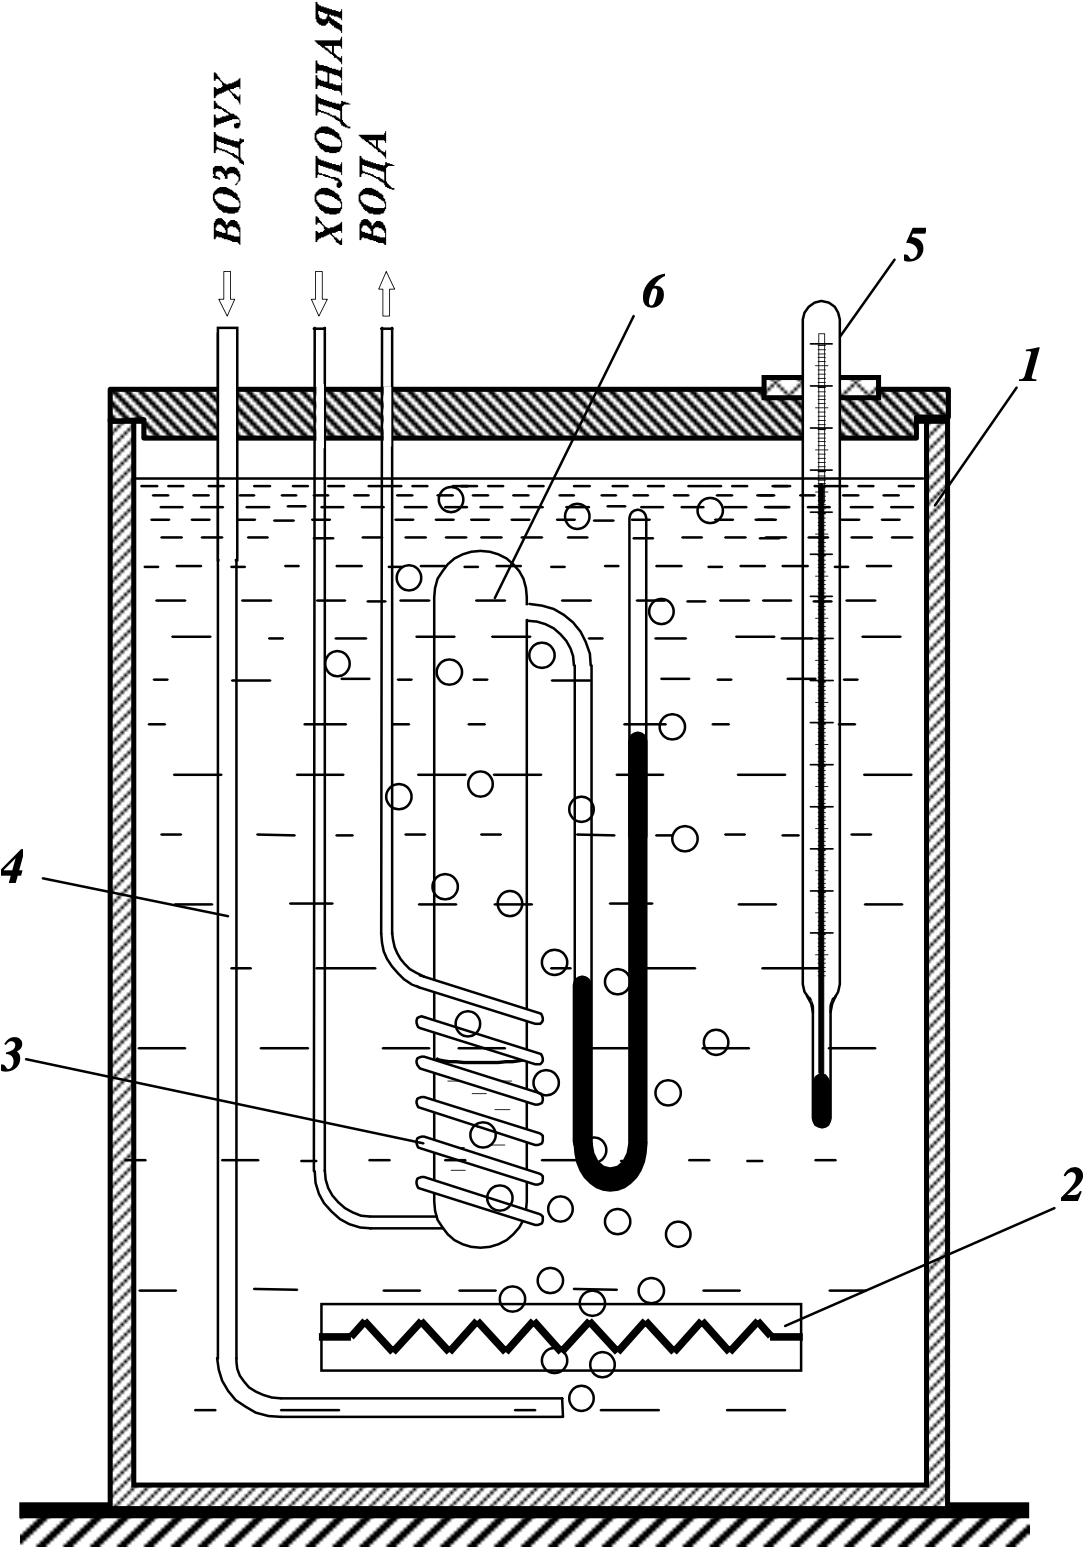
\includegraphics[width=1\linewidth]{images/ust1.png}
                \caption{Схема установки для определения теплоты испарения}
                \label{pic1}
            \end{minipage}
            \hfill
            \begin{minipage}[ht]{0.65\linewidth}
                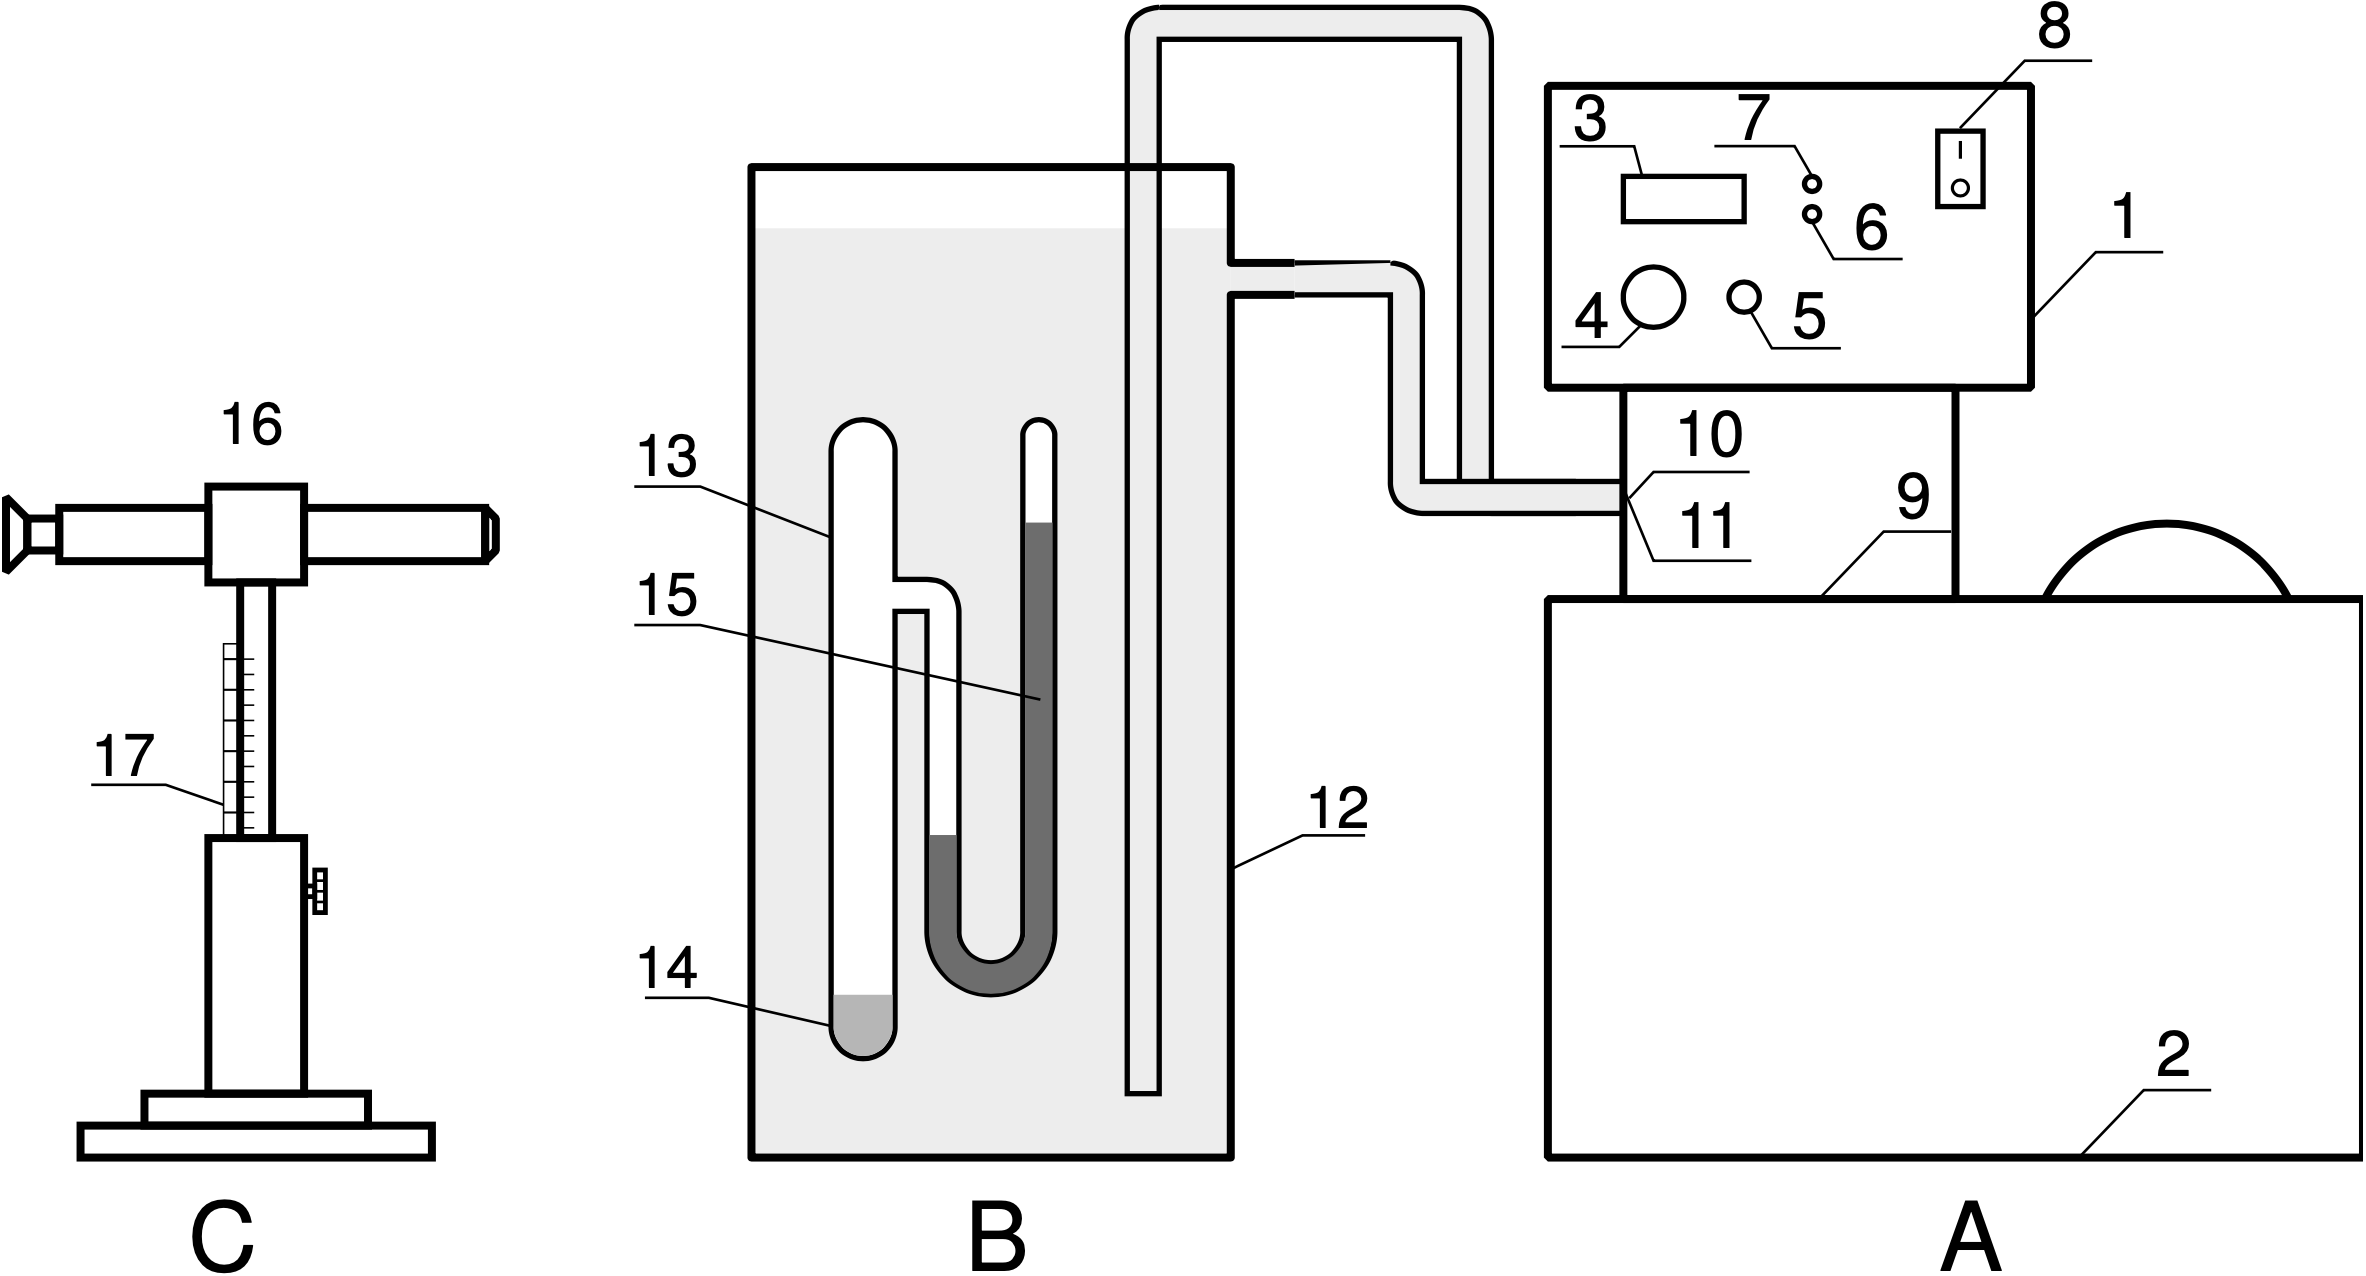
\includegraphics[width=1\linewidth]{images/ust2.png}
                \caption{Схема установки для определения теплоты испарения}
                \label{pic2}
            \end{minipage}
        \end{center}
    \end{figure}
    
    На рис. \ref{pic2} приведена более полная схема такой же установки, но с использованием современного термостата. Установка включает термостат A, экспериментальный прибор B и отсчетный микроскоп C.
    
    Экспериментальный прибор B представляет собой емкость 12, заполненную водой. В неё погружен запаянный прибор 13 с исследуемой жидкостью 14. Перед заполнением исследуемой жидкости воздух из запаянного прибора был удален, так что над жидкостью находится только её насыщенный пар. Давление пара определяется по ртутному манометру 15, соединенному с емкостью 13. Численная величина давления измеряется по разности показаний отсчетного микроскопа 16, настраиваемого последовательно на нижний и верхний уровни столбика ртути манометра. Показания микроскопа снимаются по шкале 17.
    
    Описание прибора указывает на второе важное преимущество предложенного косвенного метода измерения $L$ перед прямым. При непосредственном измерении теплоты испарения опыты нужно производить при неизменном давлении, и прибор не может быть запаян. При этом невозможно обеспечить такую чистоту и неизменность экспериментальных условий, как при нашей постановке опыта.
    
    Описываемый прибор обладает важным недостатком: термометр определяет температуру термостата, а не исследуемой жидкости (или ее пара). Эти температуры близки друг к другу лишь в том случае, если нагревание происходит достаточно медленно. Убедиться в том, что темп нагревания не является слишком быстрым, можно, сравнивая результаты, полученные при нагревании и при остывании прибора. Такое сравнение необходимо сделать. Для ориентировки укажем, что температуру воды в калориметре следует менять не быстрее, чем на 1 $^\circ\text{C}$ в течение 1–3 минут.
    
    \begin{flushleft}
        {\Large {\bf Ход работы}}
    \end{flushleft}
    
    \begin{enumerate}
    
        \item[1.] Запишем погрешности измерительных приборов:
            \begin{itemize}
                \item Термостат жидкостный ТЖ-ТС-01: $\sigma_T = \pm 0,1 \text{ } ^\circ\text{C}$
                \item Штангенциркуль: $\sigma_h = \pm 0,1 \text{ } мм$
            \end{itemize}
            
        \item[2.] Выставим температуру $T = 20 \text{ } ^\circ\text{C}$ на термостате. После её установления подождём 1,5-2 мин для установления термодинамического равновесия и с помощью микроскопа измерим разность уровней в ртутном U-образном манометре. Для уменьшения случайной погрешности разность уровней для каждой температуры будем измерять три раза. Полученные результаты усредним. Все данные будем заносить в табл. \ref{table1}.
        
        \item[3.] Повысим температуру на $\Delta T = 1 \text{ } ^\circ\text{C}$. После её установления повторим все измерения п. 2. Результаты также будем заносить в табл. \ref{table1}.
        
    \end{enumerate}
    
    \begin{table}[ht]
        \centering
        \captionsetup{justification=centering, margin=2cm}
        \begin{tabular}{||c|c||c|c||c|c||}
            \hline
            $T$, $^\circ\text{C}$ & $\Delta h_\text{ср}$, мм & $T$, $^\circ\text{C}$ & $\Delta h_\text{ср}$, мм & $T$, $^\circ\text{C}$ & $\Delta h_\text{ср}$, мм \\
            \hline
            20,0 & 15,0 & 26,1 & 18,9 & 32,0 & 28,9 \\
            \hline
            21,0 & 15,0 & 27,0 & 20,3 & 33,0 & 30,9 \\
            \hline
            22,0 & 15,4 & 28,0 & 21,9 & 34,1 & 32,8 \\
            \hline
            23,0 & 15,9 & 29,0 & 23,4 & 35,0 & 35,0 \\
            \hline
            24,0 & 16,7 & 30,0 & 25,0 & 36,1 & 37,3 \\
            \hline
            25,1 & 17,7 & 31,0 & 26,9 & 37,1 & 39,7 \\
            \hline
        \end{tabular}
        \caption{Средние значения разности уровней U-образного манометра при данных температурах}
        \label{table1}
    \end{table}
    
    \begin{flushleft}
        {\Large {\bf Обработка результатов эксперимента}}
    \end{flushleft}
    
    \begin{enumerate}
    
        \item[1.] По формуле $P = \rho g h$, где $\rho = 13596 \text{ } кг/м^3$ — плотность ртути, $g = 9,806 \text{ } м/с^2$ — ускорение свободного падения, $h$ — разность уровней U-образного манометра, и пользуясь данными табл. \ref{table1} переведём разность уровней U-образного манометра в давление насыщенного пара в Паскалях. Результат представим в табл. \ref{table2}.
        
        \begin{table}[ht]
            \centering
            \begin{tabular}{||c|c||c|c||c|c||}
                \hline
                $T$, $^\circ\text{C}$ & $P$, кПа & $T$, $^\circ\text{C}$ & $P$, кПа & $T$, $^\circ\text{C}$ & $P$, кПа \\ 
                \hline
                20,0 & 1,20 & 26,1 & 2,52 & 32,0 & 3,86 \\
                \hline
                21,0 & 1,20 & 27,0 & 2,71 & 33,0 & 4,12 \\
                \hline
                22,0 & 2,06 & 28,0 & 2,92 & 34,1 & 4,37 \\
                \hline
                23,0 & 2,12 & 29,0 & 3,12 & 35,0 & 4,67 \\
                \hline
                24,0 & 2,22 & 30,0 & 3,34 & 36,1 & 4,97 \\
                \hline
                25,1 & 2,36 & 31,0 & 3,59 & 37,1 & 5,30 \\
                \hline
            \end{tabular}
            \caption{Давления насыщенного водяного пара при данных температурах}
            \label{table2}
        \end{table}
        
        \item[2.] Построим график зависимости $\text{ln}P(1/T)$ по МНК, где T — температура в Кельвинах, и, найдя значение коэффициента наклона $d(\text{ln}P)/d(1/T)$, найдём значение теплоты испарения воды $L$ по формуле \eqref{eq4}. При построении графика выкинем несколько начальных точек, т. к. при низких температурах график имеет нелинейный вид.
        
        Погрешности рассчитаем по следующим формулам:
        \begin{equation}
            \sigma_{\Delta h_{ср}} = \sqrt{2} \sigma_h, \text{ } \varepsilon_P = \varepsilon_{\Delta h_{ср}},
        \end{equation}
        \begin{equation}
            \varepsilon_{\text{ln}P} = \varepsilon_P,
        \end{equation}
        \begin{equation}
            \varepsilon_{d(\text{ln}P)/d(1/T)}^{приб} = \sqrt{\varepsilon_{\text{ln}P}^2 + \varepsilon_{T}^2},
        \end{equation}
        \begin{equation}
            \sigma_{d(\text{ln}P)/d(1/T)} = \sqrt{(\sigma_{d(\text{ln}P)/d(1/T)}^{приб})^2 + (\sigma_{d(\text{ln}P)/d(1/T)}^{случ})^2}.
        \end{equation}
        Случайную погрешность посчитаем по МНК. Все результаты приведём в табл. \ref{table3}. \\
        
        \begin{figure}[ht]
            \centering
            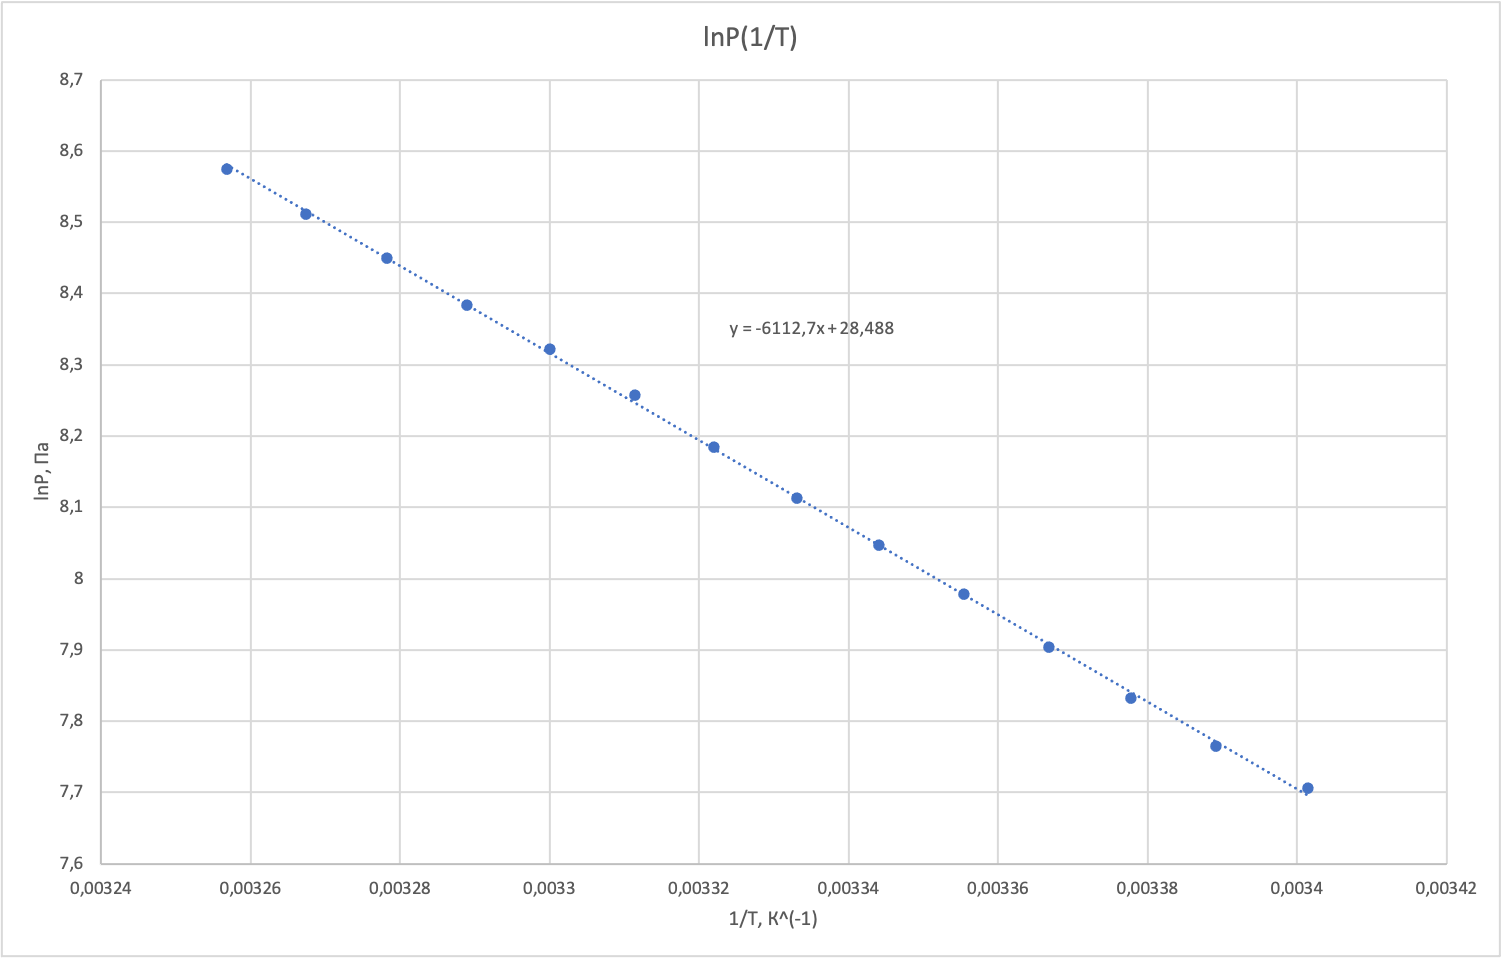
\includegraphics[width=0.75\linewidth]{images/lnP(1:T).png}
        \end{figure}
        
        \begin{table}[ht]
            \centering
            
            \begin{tabular}{|c|c|c|c|c|c|c|c|c|c|}
                \hline
                $\text{ln}P$, Па & 7,60 & 7,60 & 7,63 & 7,66 & 7,71 & 7,76 & 7,83 & 7,90 & 7,98 \\   
                \hline
                $1/T$, К$^{-1}$ & 0,00345 & 0,00344 & 0,00342 & 0,00341 & 0,00340 & 0,00339 & 0,00338 & 0,00337 & 0,00337 \\
                \hline
            \end{tabular}
            
            \vspace{0.2cm}
            
            \begin{tabular}{|c|c|c|c|c|c|c|c|c|c|}
                \hline
                $\text{ln}P$, Па & 8,05 & 8,11 & 8,18 & 8,26 & 8,32 & 8,38 & 8,45 & 8,51 & 8,58 \\
                \hline
                $1/T$, К$^{-1}$ & 0,00334 & 0,00333 & 0,00332 & 0,00331 & 0,00330 & 0,00329 & 0,00328 & 0,00327 & 0,00326 \\
                \hline
            \end{tabular}
            
            \caption{График зависимости $\text{ln}P$ от $1/T$}
            \label{table3}
        \end{table}
        
        В итоге получим
        \begin{equation}
            \frac{d(\text{ln}P)}{d(1/T)} = (-611 \pm 5) \cdot 10 \text{ } [Па \cdot К].
        \end{equation}
        
        Теперь по формуле \eqref{eq4} рассчитаем $L$. Погрешность: $\varepsilon_L = \varepsilon_{d(\text{ln}P)/d(1/T)}$. В итоге
        \begin{equation}
            L = (50,8 \pm 0,4) \text{ } кДж/моль. \\
        \end{equation}
        
    \end{enumerate}
    
    \begin{flushleft}
        {\Large {\bf Вывод}}
    \end{flushleft}
    
    В данной работе мы получили значение молярной теплоты испарения воды, а также узнали, как зависит молярная теплота испарения жидкости от температуры и давления. Получившееся значение не совпало с табличным даже в пределах погрешности. Скорее всего, это связано с тем, что температура насыщенного водяного пара не совпадала с температурой воды в термостате во время проведения эксперимента. Также на конечный результат повлияли пренебрежения, сделанные нами в нашей теоретической модели.
    
\end{document}